\documentclass[twocolumn,linenumbers]{aastex631}
%%\documentclass[linenumbers]{aastex631}
%%\documentclass[modern]{aastex631}
%%\documentclass[twocolumn]{aastex631}
\newcommand{\vdag}{(v)^\dagger}
\newcommand\aastex{AAS\TeX}
\newcommand\latex{La\TeX}

\usepackage{mathtools, graphicx, booktabs, apjfonts, soul}
%\addbibresource{Bibliography.bib} %For bibliography

\begin{document}

\title{The Distribution of Cohesive Objects in the Universe: an Extended "Main Sequence"
\footnote{Sept, 17, 2024}}

\author[0000-0002-8482-4669]{Gabriel M Steward}
\affiliation{University of Idaho, Moscow, Idaho 83844}

\author{Matthew Hedman}
\affiliation{University of Idaho, Moscow, Idaho 83844}

\begin{abstract}

\textbf{\color{red}ABSTRACTION: this will be done last, as we need to know the end from the beginning to properly do it.\color{black}}

\end{abstract}

\keywords{KEYWORDS (111) --- KEYWORDS (112)}

\section{Introduction} \label{sec:intro}

\textbf{\color{red} [NOTE: For major notes.] \color{black}}

\textbf{\color{blue}For placeholder stuff and jotted notes. \color{black}}

The HR (Hertzsprung-Russel) diagram is a familiar sight to many. The relation of color temperature to luminosity sucinctely shows how a simple relation of two components can be used to identify, categorize, and explain objects in space. The success of the HR diagram is difficult to overstate, as it is a cornerstone of astronomy or astrophysics course. 

In recent years, a similar endeavor has been undertaken for exoplanets. Now that we have over 5000 confirmed discoveries, mass/radius plots can be constructed that show distinct domains of planetary types \citep{Chen2016, Muller2024}. These graphs, while similar in purpose and scope to the HR diagram, are not yet as successful, but likely will be in the future. One can also find similar distribution graphs for asteroids, such as mass-density plots \citep{Carry2012}. 

One may be tempted to think that these three domains of stars, exoplanets, and asteroids are entirely unrelated. However, that is not the case; all of them share some simple, basic properties. All of them are cohsive objects; that is, objects that are made of components in physical contact with each other, as opposed to non-cohesive objects like nebulae or galaxies. Each cohesive object has a particular mass and size, from which density and surface gravity can be determined. This means that every one of these objects can be placed on the same plot so long as two of the aforementioned values were used. 

In this paper, we present such a graph that plots the mass-density relation for all cohesive objects that we have decent measurements for, ranging from miniscule asteroids to supermassive black holes. The intention is that this plot will be shared readily among the community as a way to examine the overall distribution of objects in the universe, connecting many disciplines across astrophysics. Like the HR diagram, this distribution plot suggests many clear divisions by which to categorize objects, and even has an extended "main sequence" of sorts on which the vast majority of objects fall. 

We begin with \textbf{Results} since the primary result of this paper is the driving force behind it. \textbf{Discussion} of the distributions come next, including classification implications, outlier examinations, and uncertainties. The \textbf{Conclusion} of our work comes next, though afterward we describe the \textbf{Methods} used to gather and pair down the data. 

\section{Results} \label{sec:intro}

\begin{figure*}[htbp]
\centering
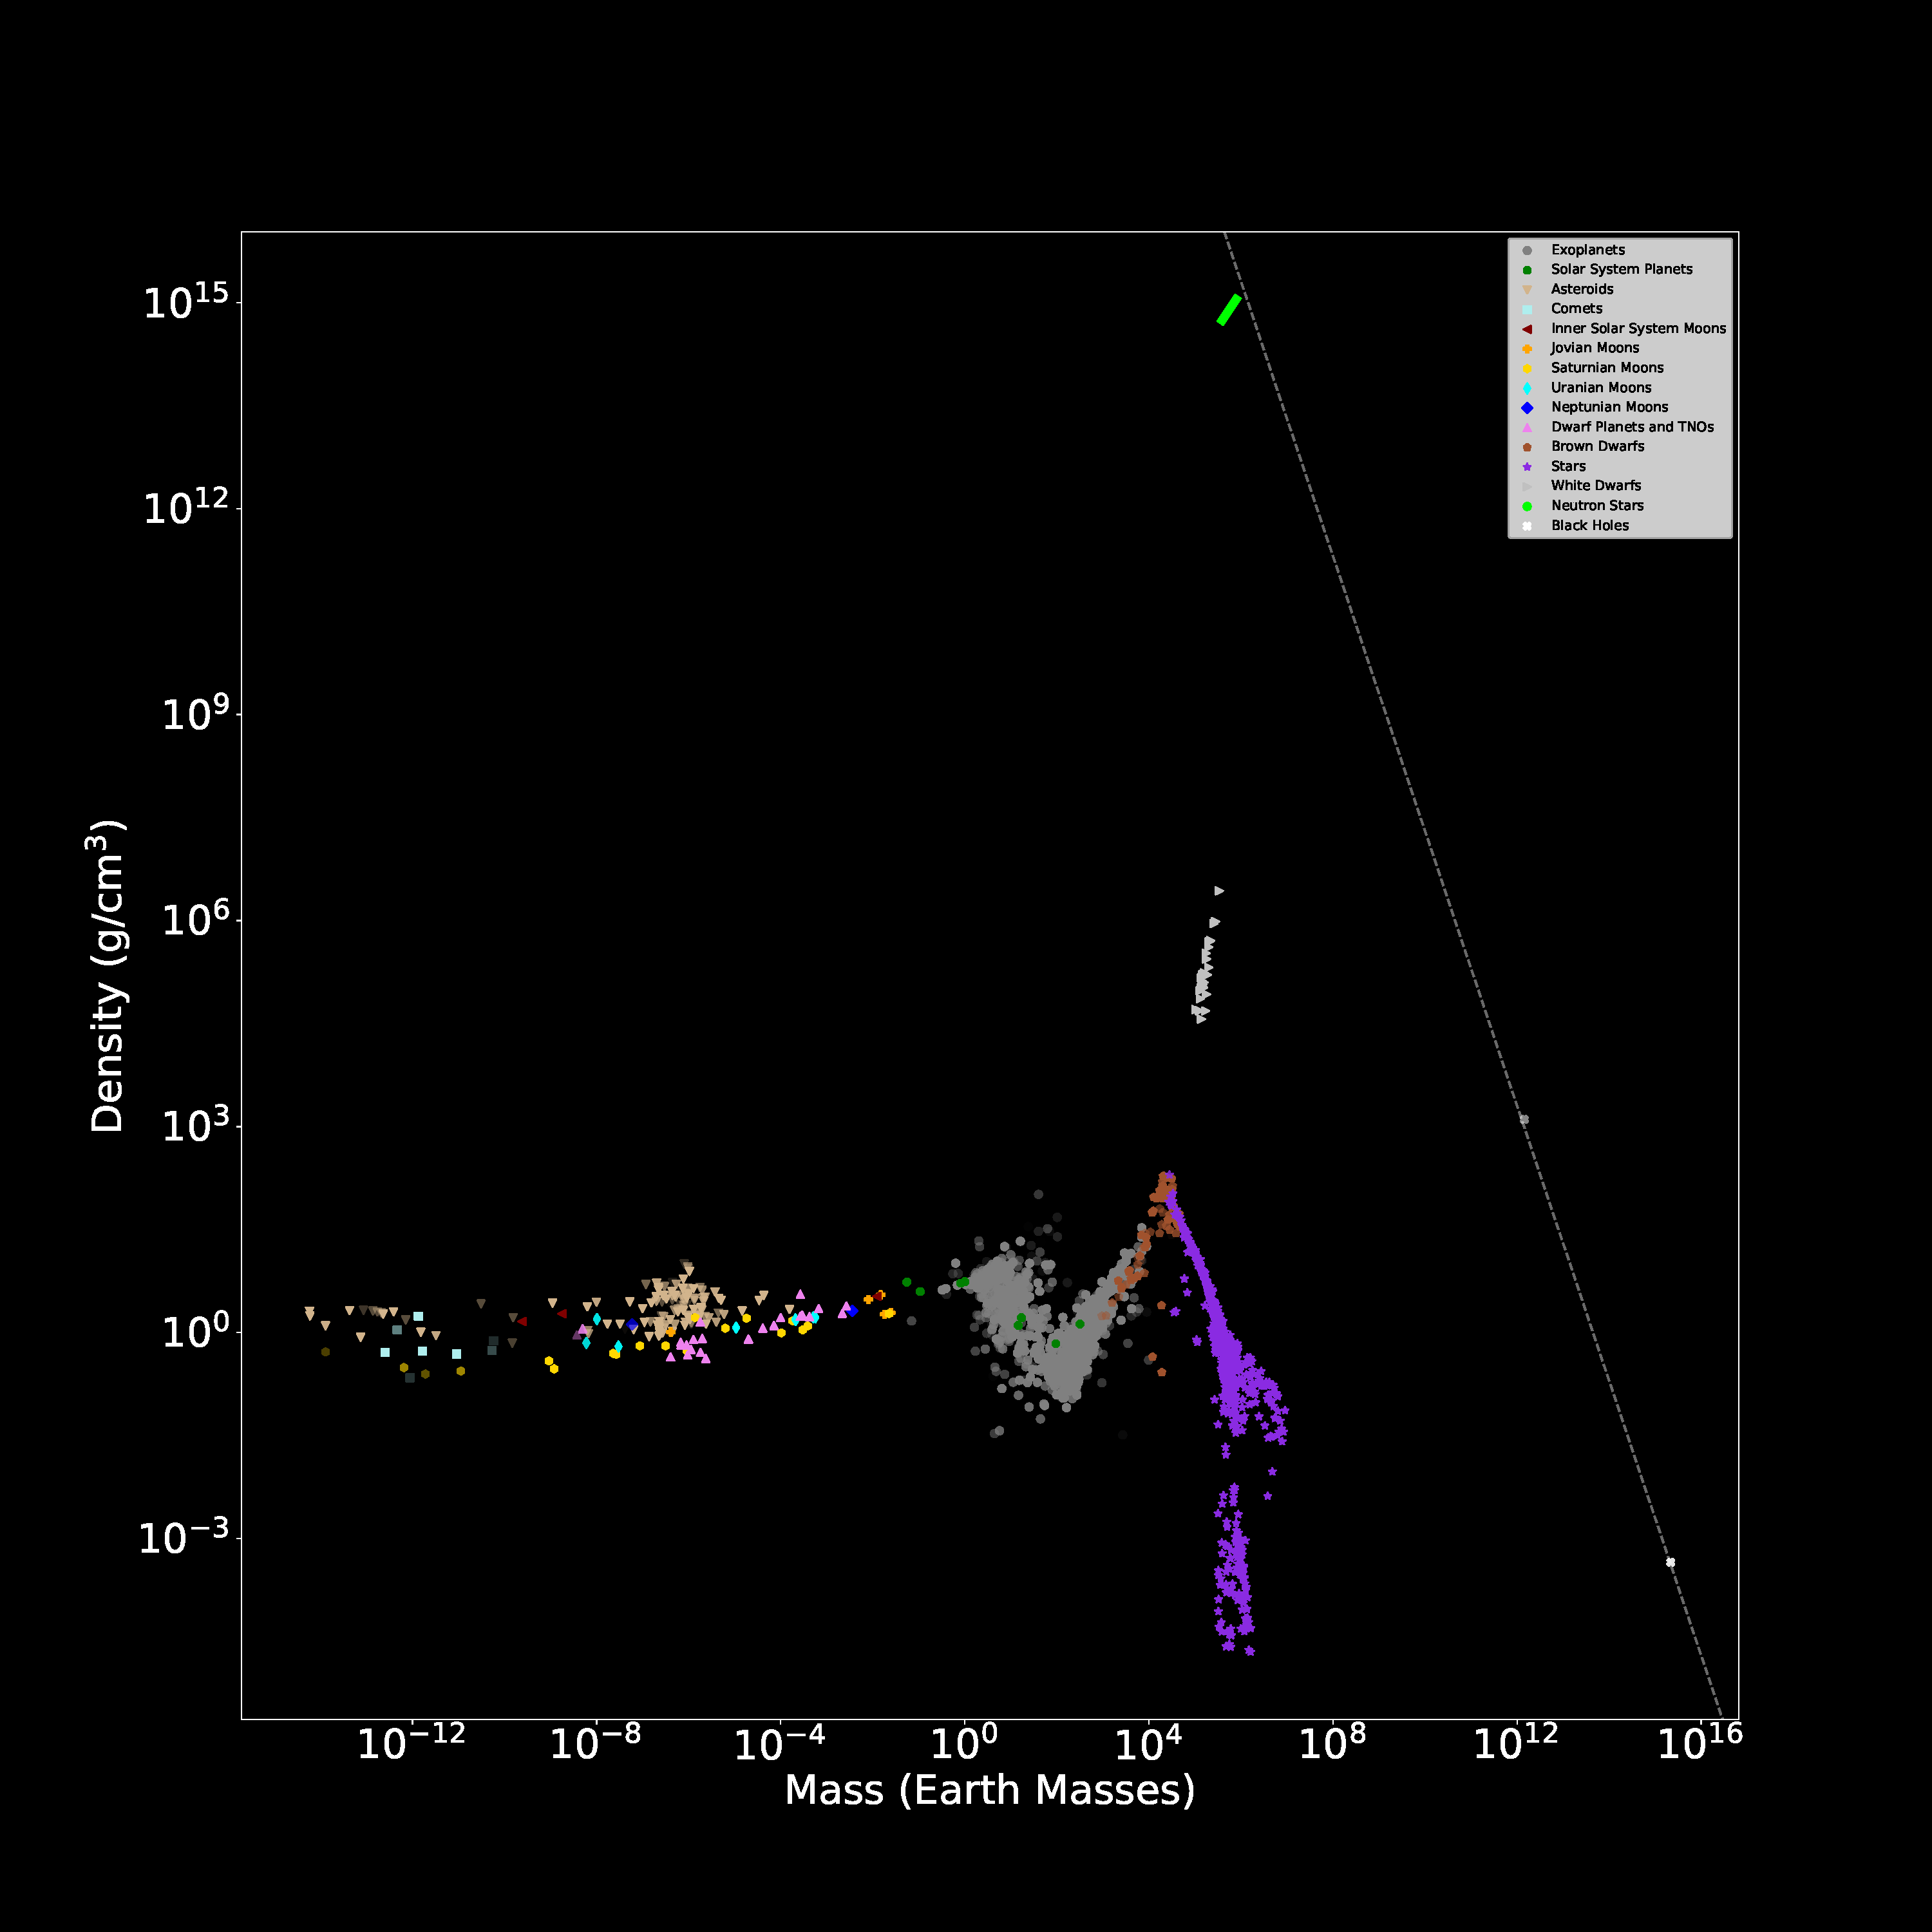
\includegraphics[scale = 0.35]{MassDensityPlot.pdf}
\centering
\caption{The relationship between density (in g/cm$^3$) and mass (in Earth masses) for cohesive objects in the universe on a log-log scale. Each kind of object is given a unique color and shape. The transparency of each point represents how large the errors are: solid objects have minimal errors while the more transparent ones have larger errors with a maximum relative permitted error of 0.5 in either mass or thrice the radius, whichever was larger for the object in question. As no  neutron star radii have been measured to precision, the general area Neutron Stars occupy is given by a green line. The dashed line represents the black hole limit, any object that reaches this line should theoretically collapse into a black hole. }
\label{fig:1}
\end{figure*}

Figure \ref{fig:1} is our primary result, showing the relation of mass and density for asteroids, comets, trans-Neptunian objects, moons, planets, brown dwarfs, stars, neutron stars, and black holes. Every data point represents a real object in the scientific literature. The points are categorized by type via shape and color, the classification assigned based on the source they were found in. This draws attention to the inconsistent distinction between exoplanets and brown dwarfs, as well of the wide vareity in exoplanets and stars. Transparency represents the relative error associated with each object: low errors plot solid points, while high errors are almost transparent. The maximum relative error plotted is 0.5 for the mass or volume, whichever was larger. Direct radius relative error was not used as mass correlates with radius cubed, and so the error propogations differ between the two by a factor of 3. The largest errors are particuarly noteworthy on outlier exoplanets, outlier asteroids, and particuarly small objects. 

No neutron stars have had their radii measured with sufficient precision as far as we are aware. Thus, a loose range of neutron star masses and densities are plotted as a fat line, rather than individual points. Two black hole event horizon radii have been satisfactorily measured, and they are on the plot, but to put them in contaxt we opted to plot the theoretical mass-density relation for Schwarzchild black holes.

Expanded views of various sections of Figure \ref{fig:1} are shown in Figure \ref{fig:2}, examing four different mass scales. These views make it possible to pick out individual objects among the otherwise dense clouds.  

\begin{figure*}[htbp]
\centering
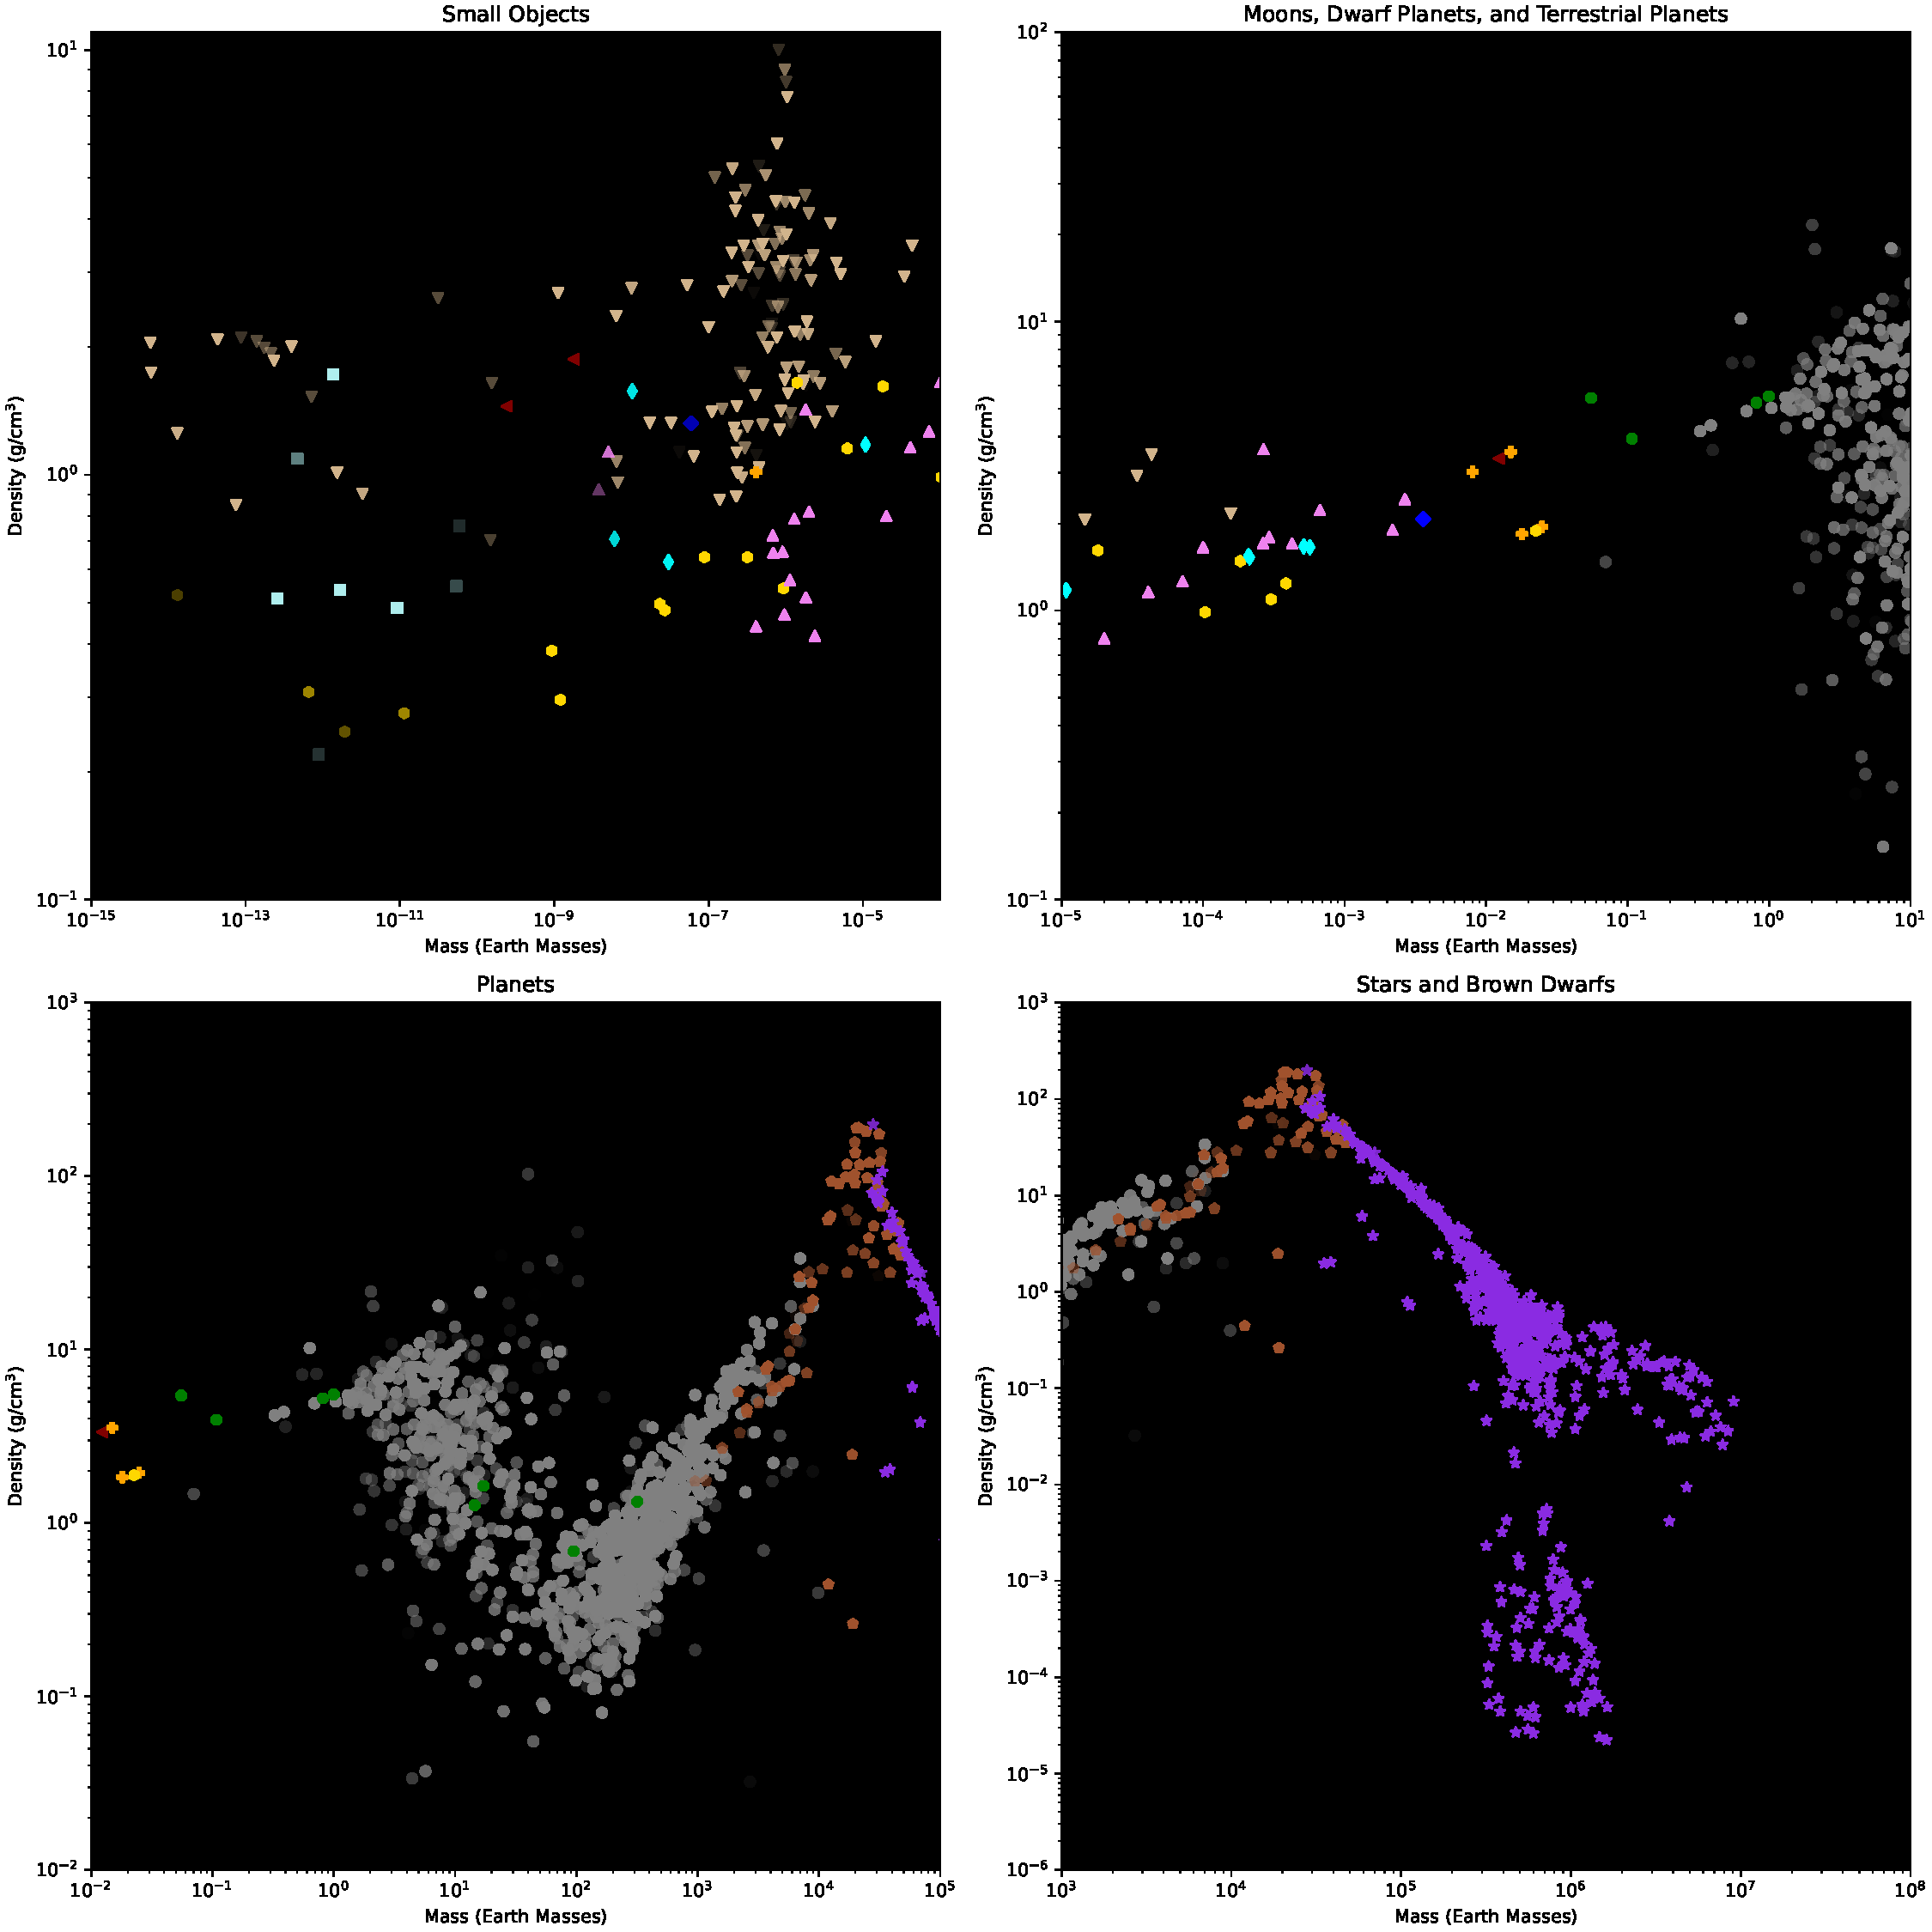
\includegraphics[scale = 0.35]{ZoomViews.pdf}
\centering
\caption{Zoomed in views of Figure \ref{fig:1} using the same colors and shapes. No view for white dwarfs or other extreme objects, as there is not much detail present in those ranges to begin with.}
\label{fig:2}
\end{figure*}

The actual data collected in our dataset are mass and radius, not mass and density. Mass and density were chosen for Figure \ref{fig:1} because it makes it easier to see distinct categories of objects, particuarly in the lower-mass regime of exoplanets. However, the mass-radius relation is not ignored; we have it plotted in Figure \ref{fig:3} alongside other combinations of mass, radius, density, and surface gravity. 

\begin{figure*}[htbp]
\centering
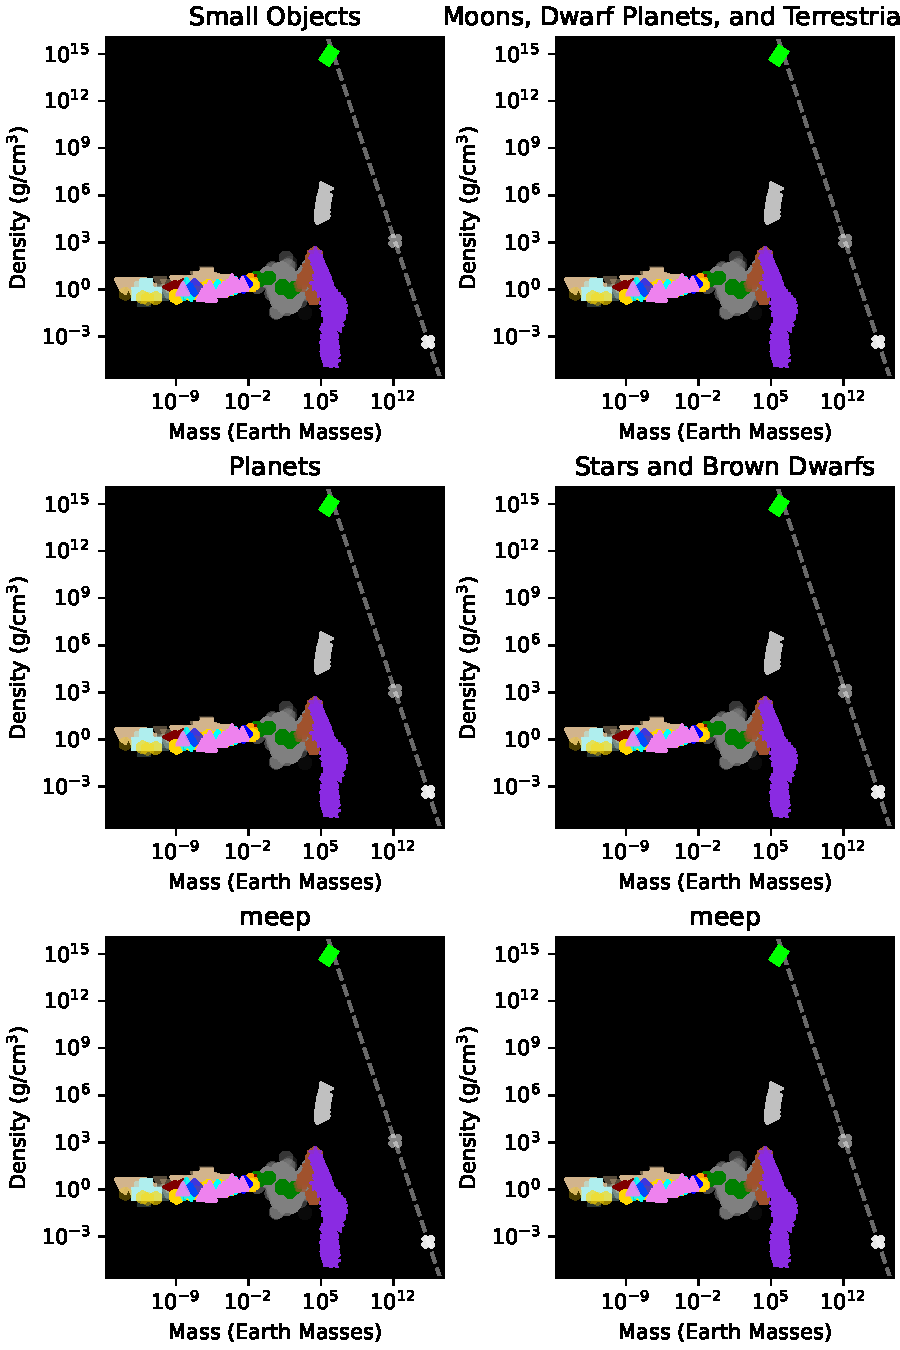
\includegraphics[scale = 1]{AltVariableViews.pdf}
\centering
\caption{Alternate views of the data set showing different combinations of mass, radius, density, and surface gravity. Colors and shapes are identical to  Figure \ref{fig:1}.}
\label{fig:3}
\end{figure*}

\section{Discussion} \label{sec:intro}

\textbf{\color{blue}DISCUSSION: Note the primary types of objects and their domains, what the "main sequence" is, what things are off of it, etc. Have a section about the outliers that survived inspection. Discuss how we can and cannot classify objects, overlaps, and questionable areas. Just have fun talking about it!\color{black}}

\section{Conclusion} \label{sec:intro}

\textbf{\color{blue}CONCLUSION: Discuss the major points, how the graph might be used, and what we can learn from it. Also note holes in the graph that could be filled in the future. \color{black}}

\section{Methods} \label{sec:methods}

Minimum neutron star \citep{Suwa2018}. 

Maximum neutron star \citep{Romani2022}. 

Neutron star radius \citep{Ozel2016}. 

TNO Test \citep{Brown2017}. 

TEST \citep{Morin2010}

\textbf{\color{blue}METHODS: In the back discuss the nitty-gritty deatils of where the data was gathered from, how it was trimmed down, and what the requirements were. Also discuss outlier handling. This is mainly where a ton of citaitons are going to go. \color{black}}

\begin{acknowledgments}
Insert ACK here. 

\textbf{\color{blue}Data availability? Would like to make it clear that we'll give all the information after just being asked...\color{black}}

\textbf{\color{red}[Not sure who needs to be put here who won't be put on the author list. Though there is going to be funding recongition here.]\color{black}}
\end{acknowledgments}

\appendix

\section{Appendix?}

Appendix!

\bibliography{Bibliography}{}
\bibliographystyle{aasjournal}

\end{document}